\documentclass{article}
\usepackage{graphicx, tikz-cd, float, titlepic, booktabs} % Required for inserting images
\usepackage{pgfplots}
\usepackage{multicol}
\usepackage{makecell}
\pgfplotsset{compat=1.15}
\usepackage{mathrsfs}
\usetikzlibrary{arrows}
\usepackage{amsmath, amssymb, amsthm, amsfonts, siunitx, physics, gensymb}
\AtBeginDocument{\RenewCommandCopy\qty\SI}
\usepackage[version=4]{mhchem}
\usepackage[most,many,breakable]{tcolorbox}
\usepackage{xcolor, fancyhdr, varwidth}
\usepackage[Glenn]{fncychap}
%Options: Sonny, Lenny, Glenn, Conny, Rejne, Bjarne, Bjornstrup
\usepackage{hyperref, cleveref}
\usepackage{icomma, enumitem} %comma as decimal and continue enumerate with [resume]
\usepackage{plimsoll} %use standard state symbol with \stst
\usepackage[danish]{babel}
\renewcommand{\cellalign}{cl}
\renewcommand{\theadalign}{cl}
\renewcommand\theadfont{\bfseries}
%%%%%%%%%%%%%%%%%%%%%%%%%%%%%%
% SELF MADE COLORS
%%%%%%%%%%%%%%%%%%%%%%%%%%%%%%
\definecolor{myg}{RGB}{56, 140, 70}
\definecolor{myb}{RGB}{45, 111, 177}
\definecolor{myr}{RGB}{199, 68, 64}
\definecolor{mytheorembg}{HTML}{F2F2F9}
\definecolor{mytheoremfr}{HTML}{00007B}
\definecolor{mylenmabg}{HTML}{FFFAF8}
\definecolor{mylenmafr}{HTML}{983b0f}
\definecolor{mypropbg}{HTML}{f2fbfc}
\definecolor{mypropfr}{HTML}{191971}
\definecolor{myexamplebg}{HTML}{F2FBF8}
\definecolor{myexamplefr}{HTML}{88D6D1}
\definecolor{myexampleti}{HTML}{2A7F7F}
\definecolor{mydefinitbg}{HTML}{E5E5FF}
\definecolor{mydefinitfr}{HTML}{3F3FA3}
\definecolor{notesgreen}{RGB}{0,162,0}
\definecolor{myp}{RGB}{197, 92, 212}
\definecolor{mygr}{HTML}{2C3338}
\definecolor{myred}{RGB}{127,0,0}
\definecolor{myyellow}{RGB}{169,121,69}
\definecolor{myexercisebg}{HTML}{F2FBF8}
\definecolor{myexercisefg}{HTML}{88D6D1}
%%%%%%%%%%%%%%%%%%%%%%%%%%%%%%%%%%%%%%%%%%%%%%%%%%%%%%%%%%%%%%%%%%%%%%
% Box environments for theorems and problems
%%%%%%%%%%%%%%%%%%%%%%%%%%%%%%%%%%%%%%%%%%%%%%%%%%%%%%%%%%%%%%%%%%%%%
\setlength{\parindent}{1cm}
%================================
% Question BOX
%================================
\makeatletter
\newtcbtheorem{question}{Opgave}{enhanced,
	breakable,
	colback=white,
	colframe=myb!80!black,
	attach boxed title to top left={yshift*=-\tcboxedtitleheight},
	fonttitle=\bfseries,
	title={#2},
	boxed title size=title,
	boxed title style={%
			sharp corners,
			rounded corners=northwest,
			colback=tcbcolframe,
			boxrule=0pt,
		},
	underlay boxed title={%
			\path[fill=tcbcolframe] (title.south west)--(title.south east)
			to[out=0, in=180] ([xshift=5mm]title.east)--
			(title.center-|frame.east)
			[rounded corners=\kvtcb@arc] |-
			(frame.north) -| cycle;
		},
	#1
}{def}
\makeatother
%================================
% DEFINITION BOX
%================================

\newtcbtheorem[]{Definition}{Definition}{enhanced,
	before skip=2mm,after skip=2mm, colback=red!5,colframe=red!80!black,boxrule=0.5mm,
	attach boxed title to top left={xshift=1cm,yshift*=1mm-\tcboxedtitleheight}, varwidth boxed title*=-3cm,
	boxed title style={frame code={
					\path[fill=tcbcolback]
					([yshift=-1mm,xshift=-1mm]frame.north west)
					arc[start angle=0,end angle=180,radius=1mm]
					([yshift=-1mm,xshift=1mm]frame.north east)
					arc[start angle=180,end angle=0,radius=1mm];
					\path[left color=tcbcolback!60!black,right color=tcbcolback!60!black,
						middle color=tcbcolback!80!black]
					([xshift=-2mm]frame.north west) -- ([xshift=2mm]frame.north east)
					[rounded corners=1mm]-- ([xshift=1mm,yshift=-1mm]frame.north east)
					-- (frame.south east) -- (frame.south west)
					-- ([xshift=-1mm,yshift=-1mm]frame.north west)
					[sharp corners]-- cycle;
				},interior engine=empty,
		},
	fonttitle=\bfseries,
	title={#2},#1}{def}
\newtcbtheorem[]{definition}{Definition}{enhanced,
	before skip=2mm,after skip=2mm, colback=red!5,colframe=red!80!black,boxrule=0.5mm,
	attach boxed title to top left={xshift=1cm,yshift*=1mm-\tcboxedtitleheight}, varwidth boxed title*=-3cm,
	boxed title style={frame code={
					\path[fill=tcbcolback]
					([yshift=-1mm,xshift=-1mm]frame.north west)
					arc[start angle=0,end angle=180,radius=1mm]
					([yshift=-1mm,xshift=1mm]frame.north east)
					arc[start angle=180,end angle=0,radius=1mm];
					\path[left color=tcbcolback!60!black,right color=tcbcolback!60!black,
						middle color=tcbcolback!80!black]
					([xshift=-2mm]frame.north west) -- ([xshift=2mm]frame.north east)
					[rounded corners=1mm]-- ([xshift=1mm,yshift=-1mm]frame.north east)
					-- (frame.south east) -- (frame.south west)
					-- ([xshift=-1mm,yshift=-1mm]frame.north west)
					[sharp corners]-- cycle;
				},interior engine=empty,
		},
	fonttitle=\bfseries,
	title={#2},#1}{def}

\newtcbtheorem{theo}%
    {Theorem}{}{theorem}
\newtcolorbox{prob}[1]{colback=red!5!white,colframe=red!50!black,fonttitle=\bfseries,title={#1}}
%================================
% NOTE BOX
%================================

\usetikzlibrary{arrows,calc,shadows.blur}
\tcbuselibrary{skins}
\newtcolorbox{note}[1][]{%
	enhanced jigsaw,
	colback=gray!20!white,%
	colframe=gray!80!black,
	size=small,
	boxrule=1pt,
	title=\textbf{Note:},
	halign title=flush center,
	coltitle=black,
	breakable,
	drop shadow=black!50!white,
	attach boxed title to top left={xshift=1cm,yshift=-\tcboxedtitleheight/2,yshifttext=-\tcboxedtitleheight/2},
	minipage boxed title=1.5cm,
	boxed title style={%
			colback=white,
			size=fbox,
			boxrule=1pt,
			boxsep=2pt,
			underlay={%
					\coordinate (dotA) at ($(interior.west) + (-0.5pt,0)$);
					\coordinate (dotB) at ($(interior.east) + (0.5pt,0)$);
					\begin{scope}
						\clip (interior.north west) rectangle ([xshift=3ex]interior.east);
						\filldraw [white, blur shadow={shadow opacity=60, shadow yshift=-.75ex}, rounded corners=2pt] (interior.north west) rectangle (interior.south east);
					\end{scope}
					\begin{scope}[gray!80!black]
						\fill (dotA) circle (2pt);
						\fill (dotB) circle (2pt);
					\end{scope}
				},
		},
	#1,
}
%================================
% EXAMPLE BOX
%================================
\newtcbtheorem[number within=section]{Example}{Example}
{%
	colback = myexamplebg
	,breakable
	,colframe = myexamplefr
	,coltitle = myexampleti
	,boxrule = 1pt
	,sharp corners
	,detach title
	,before upper=\tcbtitle\par\smallskip
	,fonttitle = \bfseries
	,description font = \mdseries
	,separator sign none
	,description delimiters parenthesis
}
{ex}
%================================
% THEOREM BOX
%================================

\tcbuselibrary{theorems,skins,hooks}
\newtcbtheorem[number within=section]{Theorem}{Theorem}
{%
	enhanced,
	breakable,
	colback = mytheorembg,
	frame hidden,
	boxrule = 0sp,
	borderline west = {2pt}{0pt}{mytheoremfr},
	sharp corners,
	detach title,
	before upper = \tcbtitle\par\smallskip,
	coltitle = mytheoremfr,
	fonttitle = \bfseries\sffamily,
	description font = \mdseries,
	separator sign none,
	segmentation style={solid, mytheoremfr},
}
{th}

%%%%%%%%%%%%%%%%%%%%%%%%%%%%%%%%%%%%%%%%%%%%%%%%%%%%%%%%%%%%%%%%%
% SELF MADE COMMANDS
%%%%%%%%%%%%%%%%%%%%%%%%%%%%%%
\newcommand{\sol}{\setlength{\parindent}{0cm}\textbf{\textit{Løsning:}}\setlength{\parindent}{1cm}}
\newcommand{\card}{\text{card}}
%%%%%%%%%%%%%%%%%%%%%%%%%%%%%%%%%
\usepackage[tmargin=2cm,rmargin=1in,lmargin=1in,margin=0.85in,bmargin=2cm,footskip=.2in]{geometry}\pagestyle{fancy}
\lhead{Minrui Kevin Zhou 3.b}
\rhead{Aflevering 40}

\title{Aflevering 40\\
{\Large \textbf{3.b mat A}}}
\author{Kevin Zhou}
\date{\today}

\begin{document}
\maketitle
\newpage
\begin{question}{Byggefirma}{}
  Et byggefirma har 5 murere og 7 tømrere ansat.
  Til en arbejdsopgave skal firmaet bruge et hold på 3 murere og 4 tømrere.
\end{question}
\sol \\
\textbf{a.}
Vi vil gerne finde ud af, hvor mange forskellige måder firamet kan udvælge holdet på.
Fra multiplikationsprincippet må det være produktet af kombinationer af udvælgelse af murere og kombinationer af udvælgelse af tømrere:
\begin{equation*}
\begin{split}
  K(5,3) \cdot K(7,4) &=10 \cdot 35 \\
  &=350
\end{split}
\end{equation*}
Altså kan holdet udvælges på 350 forskellige måder.
\begin{question}{Middagsoprydning}{}
  Til en middag er der 9 personer, hvoraf 5 er voksne og 4 er børn. Til at rydde af efter
middagen skal der bruges 3 personer, som udvælges ved at trække lod.
Sandsynligheden for, at der udvælges 3 voksne, er givet ved
$$\frac{K(5,3)}{K(9,3)}.$$
\end{question}
\sol \\
\textbf{a.}
Vi vil vise, at udtrykket for sandsynligheden er korrekt.

Lad $P$ betegne mængden af alle 3-kombinationer af mængden af personer, og lad $V$ betegne mængden af alle 3-kombinationer af mængden af voksne.
Vi betragter det symmetriske sandsynlighedsfelt $(P,\;p)$, og det er klart at $V \subset P$ er en hændelse i $P$. 
Siden der er tale om et symmetrisk sandsynlighedsfelt, så må der gælde, at sandsynligheden for $V$ må være antallet af elementer i $V$ over antallet af elementer i $P$, eller med andre ord
\begin{equation*}
\begin{split}
  P(V)=\frac{\card(V)}{\card(P)} =\frac{K(5,3)}{K(9,3)}
\end{split}
\end{equation*}
hvilket var, hvad vi ville vise.
\begin{question}{Binomialfordeling}{}
  En stokastisk variabel $X$ er binomialfordelt med antalsparameter 4 og sandsynlighedsparameter $\frac{1}{2}$.
\end{question}
\sol \\
\textbf{a.}
Vi beregner $P(X=2)$ for den binomialfordelte stokastiske variabel $X \sim b(4,\;\frac{1}{2})$. 
\begin{equation*}
\begin{split}
  P(x=2)&=K(4,2) \cdot \left(\frac{1}{2}\right) ^{2} \cdot \left(1-\frac{1}{2}\right) ^{4-2}\\
  &=6 \cdot \frac{1}{2^2} \cdot \frac{1}{2^2}\\
  &=\frac{3}{2^3}\\
  &=\frac{3}{8}
\end{split}
\end{equation*}
\textbf{b.}
Middelværdien $\mu $ for den stokastiske variabel $X$ er blot produktet af antalsparameteren $n$ og sandsynlighedsparameteren $p$.
\begin{equation*}
\begin{split}
  \mu &= n \cdot p \\
  &=4 \cdot \frac{1}{2} \\
  &=2
\end{split}
\end{equation*}
Middelværdien for $X$ er altså 2.\\[1ex]
\textbf{c.}
Vi beregner spredningen for $X$.
\begin{equation*}
\begin{split}
  \sigma &= \sqrt{n \cdot p \cdot \left(1-p\right) }\\
  &=\sqrt{4 \cdot \frac{1}{2} \cdot \left(1- \frac{1}{2}\right) } \\
  &=\sqrt{1} \\
  &=1
\end{split}
\end{equation*}
Spredningen for $X$ er altså $1$. 
\begin{question}{Normalfordeling}{}
  En stokastisk variabel $X$ er normalfordelt $X \sim N(5,3)$.
\end{question}
\sol \\
\textbf{a.}
Intervallerne for de exceptionelle udfald for $X$ er
\begin{equation*}
\begin{split}
  ]-\infty;\mu -3 \sigma ] &= \;]-\infty;5 -3 \cdot 3] = \;]-\infty;-4]\\
  [\mu + 3 \sigma; \infty[\;&=[5 + 3 \cdot 3; \infty[\;=[14; \infty[
\end{split}
\end{equation*}
Intervallerne for de exceptionelle udfald for $X$ er altså $]-\infty;-4]$ og $[14; \infty[$. \\[1ex]
\textbf{b.}
Intervallet for de normale udfald for $X$ er 
\begin{equation*}
\begin{split}
  [\mu - 2 \sigma ; \mu + 2 \sigma ]&=[5 - 2 \cdot 3 ; 5 + 2 \cdot 3]\\
  &=[-1;11]
\end{split}
\end{equation*}
Intervallet for de normale udfald for $X$ er altså $[-1;11]$.
\begin{question}{Vegetarer}{}
  Ifølge Coop Analyse lever 3,1\% af befolkningen vegetarisk. 
  Der udvælges på tilfældig måde en stikprøve på 200 personer. 
  Den stokastiske variabel $X$ angiver antallet af personer i denne stikprøve, der lever vegetarisk.
  Det antages, at $X$ er binomialfordelt med antalsparameter $n$ og sandsynlighedsparameter $p.$
\end{question}
\sol \\
\textbf{a.}
Siden stikprøven er på 200 personer, så må antalsparameteren $n$ være 200, da vi ved binomialeksperimentet gentager et Bernoulli-forsøg 200 gange. 
Ved hver af disse Bernoulli-forsøg er sandsynligheden for succes $3,1 \%=0,031$.
Altså har vi 
\begin{equation*}
\begin{split}
  n&=200\\
  p&=0,031
\end{split}
\end{equation*}
\textbf{b.}
Vi beregner sandsynligheden $P(X \leq 4)$ med CAS (se \cref{fig:4p}).
\begin{equation*}
\begin{split}
  P(X \leq 4)&=P(X=0)+P(X=1)+P(X=2)+P(X=3)+P(X=4)\\
  &\approx 0,2549 \\
  &=25,49 \%
\end{split}
\end{equation*}
Sandsynligheden for, at højst 4 personer i stikprøven lever vegetarisk er altså $25,49 \%$.
\begin{figure}[H]
\begin{center}
  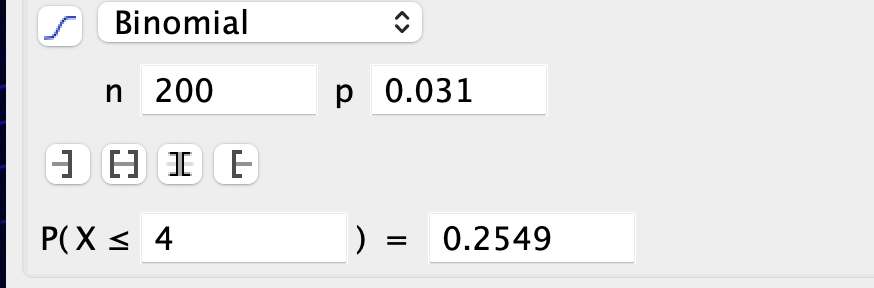
\includegraphics[width=\textwidth]{4p.png}
\end{center}
  \caption{Sandsynligheden $P(X \leq 4)$ udregnet med CAS}
\label{fig:4p}
\end{figure}
\noindent \textbf{c.}
For at finde det mest sandsynlige antal personer, der lever vegetarisk i stikprøven, beregner vi først middelværdien $\mu $.
\begin{equation*}
\begin{split}
  \mu &= n \cdot p \\
  &=200 \cdot 0,031 \\
  &=6,2
\end{split}
\end{equation*}
Det mest sandsynlige antal personer, der lever vegetarisk i stikprøven må være det ikke-negative hele tal, der er tættest på middelværdien.
Dette tal er $6$.
Ud af de 200 personer i stikprøven, er det mest sandsynlige antal personer, der lever vegetarisk altså 6.
\begin{question}{Læskedrik-maskine}{}
  Et bryggeri har en maskine, der fylder læskedrik på flasker. Maskinen er indstillet, så den mængde læskedrik, der fyldes i en flaske, er normalfordelt med middelværdi 505 mL og spredning 3 mL.
Der udtages tilfældigt 30 flasker med læskedrik ud af en dags produktion.
\end{question}
\sol \\
\textbf{a.}
Sandsynligheden for, at en læskedrik indeholder mindst $500 \;\unit{mL} $ udregnes med CAS (se \cref{fig:500mL}) og er 
\begin{equation*}
\begin{split}
  P(X \geq 500 \;\unit{mL} ) &=1-\Phi \left(\frac{500 \;\unit{mL} - \mu }{\sigma }\right) \\
  &=1- \int_{-\infty}^{\frac{500 \;\unit{mL} - 505 \;\unit{mL} }{3 \;\unit{mL} }} \left( \frac{1}{\sqrt{2 \pi } }\cdot e^{-\frac{1}{2} \cdot x^2}\right)  \,dx \\
  &\approx 0,9522 \\
  &=95,22 \%
\end{split}
\end{equation*}
Sandsynligheden for, at en tilfældigt valgt flaske med læskedrik indeholder mindst $500 \;\unit{mL} $ er altså $95,22 \;\%$. 
\begin{figure}[H]
\begin{center}
  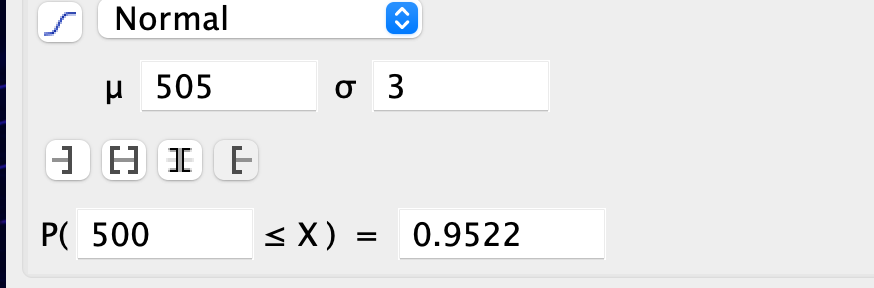
\includegraphics[width=\textwidth]{500mL.png}
\end{center}
  \caption{Sandsynligheden $P(X \geq 500 \;\unit{mL} )$ udregnet med CAS }
\label{fig:500mL}
\end{figure}
\noindent \textbf{b.}
Vi ser, at der ved, om 30 udtagne flasker indholder mindst $500 \;\unit{mL} $ læskedrik, er tale om kombination af uafhængige hændelser.
Sandsynligheden for, at alle flasker indeholder mindst $500 \;\unit{mL} $ læskedrik må derfor være
\begin{equation*}
\begin{split}
  P(X \geq 500 \;\unit{mL} ) ^{30}&\approx 0,95220965 ^{30}\\
  &\approx 0,2301\\
  &=23,01\;\%
\end{split}
\end{equation*}
Sandsynligheden for, at alle de 30 udtagne flasker indholder mindst $500 \;\unit{mL} $ læskedrik er altså $23,01\;\%$. 
\end{document}
